
The vertices $\vec{P}$ and $\vec{U}$ are
\begin{align}
    \vec{P} = \myvec{0\\0}, \vec{U} = \myvec{PU\\0} = \myvec{6.5\\0
    }
\end{align}
Let $\angle{UPM} = \theta_1$ and  $\angle{JPU} = \theta_2$
\begin{align}
    \cos{\theta_1} &= \frac{5^2+6.5^2-4^2}{2(5)(6.5)}\\
    &=0.7884\\
    \implies \theta_1 &= 37.958^{\circ}\\
    \sin{\theta_1} &= 0.615\\
    \cos{\theta_2} &= \frac{6.5^2+4.5^2-3.5^2}{2(6.5)(4.5)}\\
    &= 0.8589\\
    \implies \theta_2 &= 30.798^{\circ}\\
    \sin{\theta_2} &= 0.512
\end{align}
Now, the vertices $\vec{M}$ and $\vec{J}$ can be expressed in polar coordinate form as
\begin{align}
    \vec{M} &= 5\myvec{\cos{\theta_1}\\\sin{\theta_1}}\\
    &= \myvec{3.942\\3.075}\\
    \vec{J} &= 4.5\myvec{\cos{\theta_2}\\-\sin{\theta_2}}\\
    &= \myvec{3.865\\-2.304}
\end{align}

%%%%%%%%
\begin{tikzpicture}[scale=1]



%Marking coordiantes
\coordinate [label=above:$M$] (M) at (3.942,3.075);
\coordinate [label=below:$J$] (J) at (3.865,-2.304);
\coordinate [label=right:$U$] (U) at (6.5,0);
\coordinate [label=left:$P$] (P) at (0,0);

%Drawing triangle ABC
\draw (P) -- node[above] {6.5} (U) -- node[above] {4} (M) -- node[above] {5} (P) -- node[below] {4.5}(J) -- node[below] {3.5} (U);


%Drawing and marking angles
\tkzMarkAngle[fill=orange!40,size=0.5cm,mark=](U,P,M)
\tkzLabelAngle[pos=0.85](U,P,M){$\theta_1$}
\tkzMarkAngle[fill=orange!40,size=0.9cm,mark=](J,P,U)
\tkzLabelAngle[pos=1.3](J,P,U){$\theta_2$}
\end{tikzpicture}

\begin{figure}[!h]
 \centering
 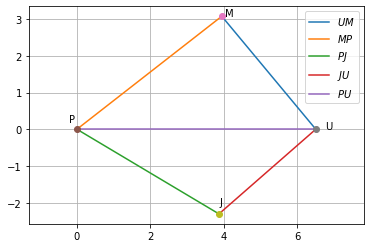
\includegraphics[width=\columnwidth]{solutions/aug/2/3/figs/Assignment3.png}
 \caption{Plot using python}
 \label{aug/2/3/plot}
\end{figure}


